\documentclass[12pt]{article}
\usepackage{blindtext}
\usepackage[utf8]{inputenc}
\usepackage{geometry}
\usepackage{graphicx}
\usepackage{xcolor}
\usepackage{amsmath}
\usepackage{amssymb}
\usepackage{graphicx}
\usepackage[export]{adjustbox}
\usepackage{fancyhdr}
\usepackage{listings}
\usepackage{multicol}
\usepackage{rotating}
\usepackage{textcomp}

%%novalidate

\usepackage{tikz}
\usepackage{calc}
\usepackage{booktabs}
%\usepackage{hyperref}

% colors
\definecolor{color1}{HTML}{770000}
%\definecolor{color1}{HTML}{8C260F}
\definecolor{color2}{HTML}{333333}


% fonts
\usepackage{fontspec}
\defaultfontfeatures{Mapping=tex-text}
\setmainfont
[Path = fonts/,
BoldFont=Lato-Bold.ttf,
ItalicFont=Lato-Italic.ttf,
BoldItalicFont=Lato-BoldItalic.ttf]
{Lato-Regular.ttf}
\newfontfamily\headingfont[Path = fonts/, ItalicFont=Lato-BlackItalic.ttf]{Lato-Black.ttf}
%%%

\usepackage{geometry}
\geometry{letterpaper,
hmargin=1in,vmargin=1in,
head=0ex,foot=4ex}

\linespread{1.5}

\usepackage[hang]{caption}
\DeclareCaptionFormat{upper}{#1#2\uppercase{#3}\par}
\captionsetup{labelfont={bf,color=color2},textfont={normalsize,color=color2},format = upper,figurename=FIGURE,tablename=TABLE}

%%% fancy sections
\usepackage{titlesec}
%\titleformat{\chapter}{\headingfont\LARGE\bfseries\scshape\color{color1}}{\thechapter}{1em}{}[\titlerule]
\titleformat{\section}{\color{color1}\headingfont\Large\bfseries\uppercase}{\thesection}{1em}{}[\titlerule]
\titleformat{\subsection}{\color{color1}\headingfont\large\bfseries\uppercase}{\thesubsection}{1em}{}
\titleformat{\subsubsection}{\color{color1}\headingfont\bfseries\uppercase}{\thesubsubsection}{1em}{}
%%%

% head and foot
\usepackage{fancyhdr}
\pagestyle{fancy}
\lhead{}
\chead{}
\makeatletter
\rhead{\color{color2}\@date}
\makeatother
\newlength{\myheight}
\lfoot{
\settoheight{\myheight}{\thepage}
\raisebox{-1ex-0.5\myheight}{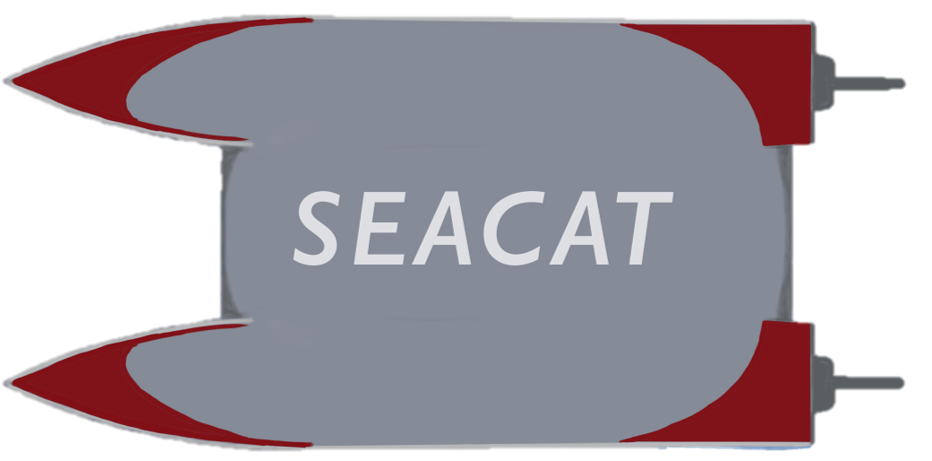
\includegraphics[height=4ex]{images/SEACAT-logo-v2.png}}
}
\cfoot{\color{color2}SEACAT Monthly Progress Report}
\rfoot{\color{color2}\thepage}
\renewcommand\headrulewidth{0pt}
\renewcommand\footrulewidth{0pt}

%%% picture on cover page
\usepackage{eso-pic}
\newcommand\BackgroundPic{%
\put(0,0){%
\parbox[b][\paperheight]{\paperwidth}{%
\vfill
\centering
\includegraphics[width=\paperwidth,height=\paperheight,%
keepaspectratio]{cover}%
\vfill
}}}
%%%
% custom titlepage
\makeatletter
\renewcommand{\maketitle}{
\thispagestyle{empty}
% \AddToShipoutPicture*{\BackgroundPic}
% \ClearShipoutPicture
\begin{center}
    
\includegraphics[]{images/panther-boat-logo-v6.png}
\end{center}
%
\phantom{a}
\vfill
\phantom{a}\hfill
\begin{tabular}[c]{@{}p{0.7\textwidth}@{}}
      \color{black}\headingfont\LARGE\@title\\[1em]
      \color{black}\headingfont\Large\@author\\[2em]
\end{tabular}
%
\clearpage
}
\makeatother
%%%


%%% fancy boxes
\usepackage{tcolorbox}
\usepackage{wrapfig}
\def\fullboxbegin{
\bigskip
\begin{tcolorbox}[colback=color1,colframe=color1,coltext=white,arc=0mm,boxrule=0pt]
}
\def\fullboxend{\end{tcolorbox}\medskip}
%
\def\leftboxbegin{
\begin{wrapfigure}{l}{0.5\textwidth}
\begin{tcolorbox}[colback=color1,colframe=color1,coltext=white,arc=0mm,boxrule=0pt]
}
\def\leftboxend{
\end{tcolorbox}
\end{wrapfigure}
}
%
\def\rightboxbegin{
\begin{wrapfigure}{r}{0.5\textwidth}
\begin{tcolorbox}[colback=color1,colframe=color1,coltext=white,arc=0mm,boxrule=0pt]
}
\def\rightboxend{
\end{tcolorbox}
\end{wrapfigure}
}
%
\newcounter{frames}
\def\frameboxbegin#1{
\bigskip
\refstepcounter{frames}
\begin{tcolorbox}[colback=white,colframe=color1,arc=0mm,title={\MakeUppercase{\textbf{Frame \arabic{frames}}: #1}}]
}
\def\frameboxend{
\end{tcolorbox}
}
%%%

\title{SEACAT Progress Report}
\author{
\\
    Braidan Duffy, Alexander Paluzzi, Sydney Cordeiro, AJ Saad\\ 
    Haylie Garman, Cannon Bogar, Mary Walker, Humberto Lebrón }
    
\date{February 2023}

\begin{document}

\maketitle

\tableofcontents 
\pagebreak

\setlength\parskip{1em plus 0.1em minus 0.2em}
% \setlength\parindent{0pt}

\section*{From the Principal Investigator} % Braidan
    Another month has passed by and things continue to progress smoothly with SEACAT.
    On February 2, we had a successful showcase of the SEACAT mockup to potential stakeholders and investors at the grand opening of the Florida Tech Mertens Center for Marine Science.
    We were invited by the Office of Development to talk about our project and meet with interested sponsors.
    Many of the alumni, board members, and visitors were impressed with our work so far and we had many good conversations over dinner!
    I want to thank Sydney, Cannon, and Humberto for their work in prepping, painting, and assembling the mock-up hulls.
    I also want to thank Haylie, Alex, and Humberto (again) for attending the Mertens opening ceremony with me and interacting with the business men and women who were interested in our mission.
    They took charge in pitching the project and fielding many of the resulting questions.

    With the conclusion of the opening ceremony, the team began Sprint 3 with, admittedly, an unclear goal in mind. 
    Compared with Sprint 2 - which had the very real deadline of the Mertens opening, Sprint 3 languished in both time spent and productivity.
    During the sprint review meeting, the team determined that we need to have a demonstration that needs to be achieved by every sprint.
    Not only will this keep us motivated, but it will also hold us accountable as we can invite stakeholders and investors to these demonstrations to show off our progress.

    So, for Sprint 4, we set out to build a demonstration for the controls system and prepare a presentation for the Introduction to Ocean Engineering class.
    This class is made up of second-semester freshmen that are oblivious to what they want to do with their academic and professional careers.
    Selfishly, we hope that these students will be inspired to join the team during our next recruiting cycle in August and give us the personnel to expand the scope and complexity of the 2023-24 boat.
    I would like to thank Sydney, Alex, Haylie, and Humberto for their work on this presentation and helping get the next generation involved.
    I would also like to thank AJ and Humberto for their diligent work on the controls system demonstration and ensuring that we could take the first steps in moving SEACAT for real.

    Going into March 2023, we are expecting to get a lot done quickly.
    First, at the end of Sprint 5 we are expecting to give our Preliminary Design Review to the PEP competition organizers, our stakeholders, investors, and other PEP competitors.
    A core tenant of my attitude with this competition carries over from my days in the FIRST\textregistered Robotics Challenge. 
    \emph{Gracious Professionalism}\textregistered  and the spirit of \emph{Coopertition}\textregistered means that we need to compete as hard as we can with our competition, but not to either of our detriment.
    It is important to acknowledge that all the competitors are just teams of students trying to learn or improve technology.
    Therefore, we must be as willing to cooperate on our innovations and share our experiences.
    By doing so, we will foster community with our adversaries and the shared knowledge between us will strengthen our individual innovations.

    It is my hope that by continuing these principles we can grow relations with new schools and form bonds and friendships that will open opportunities in the future as well as promote beneficial technology to society as a whole.
    I am pleased with what this team has done so far, and I am very excited to see it go into the future and do great things!
    
    \hspace{0.2\textwidth} Respectfully, \\
    \hspace*{0.3\textwidth}\phantom{Respectfully, }\hrulefill \\
    \hspace*{0.3\textwidth}\phantom{Respectfully, }Braidan Duffy, M.S. '23, B.S. '21 \\
    \hspace*{0.3\textwidth}\phantom{Respectfully, }Principal Investigator
\pagebreak

\section{Milestone Updates} % Alex and Sydney
    The team has completed sprints 1 through 4.
This month we achieved two milestones: 1. a showcase presentation at the Mertens Center for Marine Science and 2. a Controls Systems demonstration for the Introduction to Ocean Engineering class.
In the next two sprints, we expect to give our PDR to the competition organizers at ASNE and our stakeholders and investors. 
We are also expecting to perform tow testing on the prototype boat to observe its performance.

\begin{figure}[!h]
    \centering
    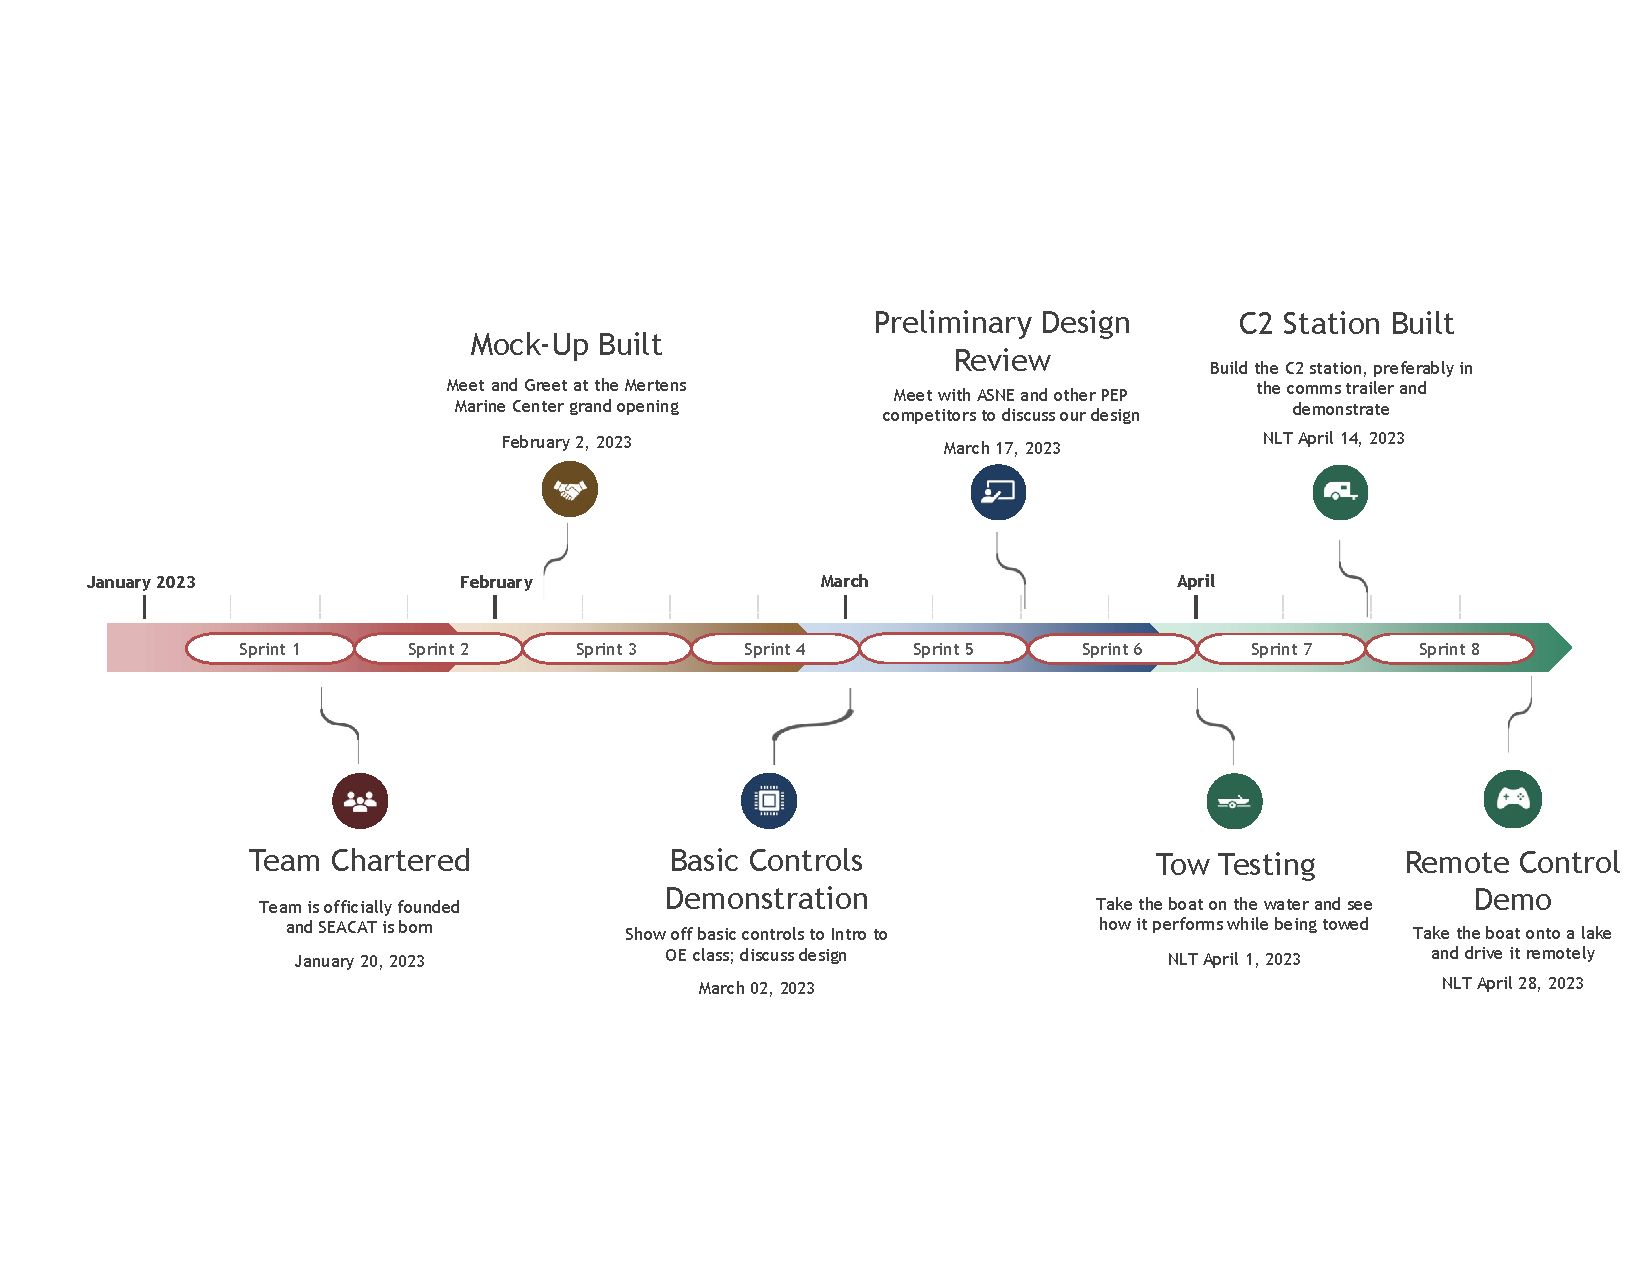
\includegraphics[width=\textwidth+0.5in]{images/02-2023/PANTHER Timeline.pdf}
    \caption{PANTHER Electric Boat milestone timeline through April 28, 2023}
    \label{fig:milestone_timeline}
\end{figure}
\pagebreak

\section{Background Research}
\subsection{CAN Overview} % Duffy and AJ
Controller Area Network (CAN) is a serial communications protocol that supports distributed real time control with high level security (cite: BOSCH CAN Specification), and is typically used to interconnect a network of modules or nodes using a two wire, twisted pair cable. 
CAN is a multimaster, multicast protocol; provided the bus is free, any node can send a message (multimaster) and all nodes can receive and act upon a message (multicast). 
The node initiating messaging is denoted as the transmitter, and any node not sending a message is called a receiver. 
CAN messages are up to 8 bytes of data and contain no explicit addresses. 
Rather, messages can be considered to be contents-addressed, where their contents determine their address. 
A message identified is used to describe the data contents which receivers can choose to use or ignore. 
While there is no method for sending a message to a specific node, hardware can provide local filtering that allows individual nodes to react only to relevant messages.
Each message is also assigned a static priority.
When a transmitter is using the bus, it is still classified as a transmitter until the bus idles or the transmitter is supplanted by another node with a higher priority.
This methodology is called arbitration and prevents messages from being transmitted over top each other.

At a high level, CAN can be subdivided into three distinct layers:

\begin{enumerate}
    \item CAN object layer
    \item CAN transfer layer
    \item Physical layer
\end{enumerate}

The object and transfer layers are composed of the services and functions of the data link layer. The object layer functionality includes:

\begin{itemize}
    \item Finding which messages are to be transmitted 
    \item Deciding which messages received by the transfer layer are to be used
    \item Provide an interface to the application layer related hardware
\end{itemize}

In the object layer, each message transmitted over the CAN bus is represented by a CAN frame, which includes several fields, such as:
\\ \\
\textbf{Identifier field}: Identifies the source and destination nodes for the message. The identifier field is a 11-bit or 29-bit field (in extended CAN) in the CAN message frame that identifies the message's priority and contents. It is used by the receiving device to determine how to handle the message. In a standard CAN message, the identifier field is 11 bits long and consists of two parts: the identifier and the remote transmission request (RTR) bit. The identifier is used to identify the message's priority and contents, while the RTR bit is used to indicate whether the message is a request for data or a message containing data.
The identifier field is used by the receiving device to determine how to handle the message. The priority of the message is determined by the identifier value, with lower values indicating higher priority. The RTR bit is used to distinguish between requests for data and messages containing data. If the RTR bit is set, the message is a request for data and the receiving device should respond with a message containing the requested data.
In an extended CAN message, the identifier field is 29 bits long and consists of three parts: the identifier, the extended identifier bit, and the RTR bit. The identifier and RTR bit are the same as in the standard CAN message, but the extended identifier bit is used to indicate that the identifier field contains an extended identifier.
\\ \\
\textbf{Data field}: Contains the actual data being transmitted. The data field of a CAN message frame can contain up to 8 bytes of data. This data can represent anything that needs to be transmitted between devices, such as sensor data, commands, or status information. The data is stored in a contiguous array of bytes, with each byte representing 8 bits of information.

The actual meaning of the data in the message depends on the application that is using the CAN bus. For example, if the CAN bus is being used to transmit sensor data, each byte of the data field may represent a different sensor value, and the values may need to be combined or interpreted in a specific way by the receiving device to make sense of the data.

It's worth noting that not all CAN messages need to have data in the data field. Some CAN messages may be used only for signaling or control purposes, and may not contain any actual data. In this case, the data field would be empty, and the length of the data field in the CAN message frame would be 0.
\\ \\
\textbf{Control field}: Contains information about the type of message and any error conditions that may be present. The control field in a CAN message frame is a 6-bit field that contains several control bits used to manage the transmission and reception of messages on the CAN bus. The control field includes the following bits:


\begin{itemize}
    \item \textbf{Data Length Code (DLC)}: A 4-bit field that specifies the length of the data field in bytes. The DLC value can range from 0 to 8 bytes.
    \item \textbf{Reserved Bit}: A reserved bit that is set to 0 and should be ignored by the receiving device.
    \item \textbf {Remote Transmission Request (RTR)}: As mentioned earlier, this bit is used to distinguish between data frames and remote frames. If the RTR bit is set, it indicates that the message is a request for data.
    \item \textbf{Identifier Extension Bit (IDE)}: In an extended CAN message, this bit is set to 1 to indicate that the identifier field contains a 29-bit extended identifier. In a standard CAN message, this bit is set to 0.
    \item \textbf{Error State Indicator (ESI)}: This bit is set to 1 by the transmitting device to indicate that an error occurred during the previous transmission. It is used to synchronize the error state between devices on the bus.
    \item \textbf{R0 and R1}: Reserved bits that are set to 0 and should be ignored by the receiving device.
\end{itemize}

    The control field is used by both the transmitting and receiving devices to manage the transmission and reception of messages on the bus. The DLC and RTR bits are particularly important, as they determine the length of the message and whether it is a request for data or a message containing data. The IDE bit is used in extended CAN messages to indicate that the identifier field contains an extended identifier. The ESI bit is used to synchronize the error state between devices on the bus. The reserved bits should always be set to 0 and ignored by the receiving device.

The object layer can also define custom messages and message formats that are specific to a particular application. 
For example, in an autonomous surface vehicle, the object layer might define messages that are used to transmit data from the vehicle's sensors to its on-board computer, or messages that are used to control the vehicle's actuators.
The transfer layer is predominately concerned with the transfer protocol.
That is, determining bus availability, starting a new transmission, or handling an incoming message. 
It delivers messages received to the object layer and accepts messages transmitting from it. 
The transfer layer also directs bit timing and synchronization, message framing, arbitration, acknowledgement, error detection/signalling, and fault confinement.

The physical layer of the CAN bus is responsible for the physical aspects of the communication. 
It includes the electrical characteristics of the communication medium, such as the voltage levels, signaling rates, and cable impedance. 
The physical layer also includes the connectors, wiring, and termination resistors used to connect the nodes on the network. 
This also incorporates the physical addressing scheme used to identify the nodes on the network. Each node is assigned a unique identifier, which is used to identify the source and destination of the messages being transmitted.

 Each node is connected to a two-wire bus, which consists of a CAN-High (CANH) and CAN-Low (CANL) wire.  These wires are used to transmit differential signals that are used to represent the bits in the packet. 
 For a logical 0 or "dominant" bit, the low and high sides are driven away from each other, increasing the voltage potential between them.
 For a logical 1 or "recessive" bit, the low and high sides are driven closer together, reducing the voltage potential. When a recessive bit (logical 1) is transmitting, both CAN-High and CAN-Low are driven to 2.5 volts (indicating the voltage difference is zero during transmission of the recessive bit); when a dominant bit (logical 0) is transmitted, CAN-High goes to 3.5 volts and CAN-Low to 1.5 (voltage difference of the dominant bit is 2 volts. If two nodes attempt to publish on the bus simultaneously, the dominant bit will be selected through arbitration (the lower the value of the identifier, the higher priority to win arbitration, publishing data on the bus.
 An example of this can be seen in the figure below:
 
 \begin{figure}[!h]
    \centering
    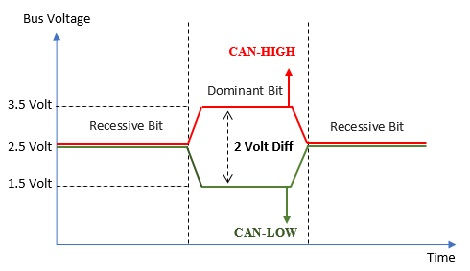
\includegraphics[width=\textwidth]{images/02-2023/CAN Differential signal.jpg}
    \caption{(Avatefipour et al., 2018) CAN bus bit transition and signal voltages}  
    \label{fig:can_specification}
\end{figure}
 When a node on the CAN bus wants to transmit a message, it first checks if the bus is idle. 
 If the bus is idle, the node can start transmitting its message. 
 The message is transmitted as a series of frames, each of which consists of seven fields:

 \begin{enumerate}
    \item \textbf{Start-of-frame (SOF)}: A single dominant bit that signals the start of a frame. 
    This bit is used to synchronize the receiving node's clock with the transmitting node's clock.
    \item \textbf{Arbitration field}: The identifier field of the frame, which includes the identifier of the message being transmitted, and is used to determine message priority during arbitration. 
    The identifier is typically a standard 11 bits (CAN 2.0A specification) or an extended 29 bits (CAN2.0B) long.
    \item \textbf{Control field}: The control field of the frame includes information about the type of message being transmitted and any error conditions.
    It contains several subfields, including the data length code (DLC) field, which specifies the number of bytes of data being transmitted and the request flag, which prompts the receiver to send a packet with the same message identifier. 
    \item \textbf{Data field}: The data field of the frame includes the actual data being transmitted, which can be up to 8 bytes long.
    \item \textbf{CRC field}: The cyclic redundancy check (CRC) field, which is used to detect errors in the message. 
    The transmitter node calculates a CRC value based on the contents of the arbitration, control, and data fields, and includes this value in the frame.
    The receiver node performs the same calculation and compares the calculated CRC value to the value received in the CRC field to check for errors.
    \item \textbf{Acknowledge (ACK) field}: The acknowledge field signals that the message has been received correctly. 
    If the message is received without errors, the receiving node sends a dominant ACK bit back to the transmitting node. 
    If an error is detected, the receiving node sends a recessive ACK bit back to the transmitting node.
    \item \textbf{End-of-frame (EOF)}: A series of seven recessive bits that signal the end of the frame.
 \end{enumerate}

 This message format is summarized in the following figure:
 
 \begin{figure}[!h]
    \centering
    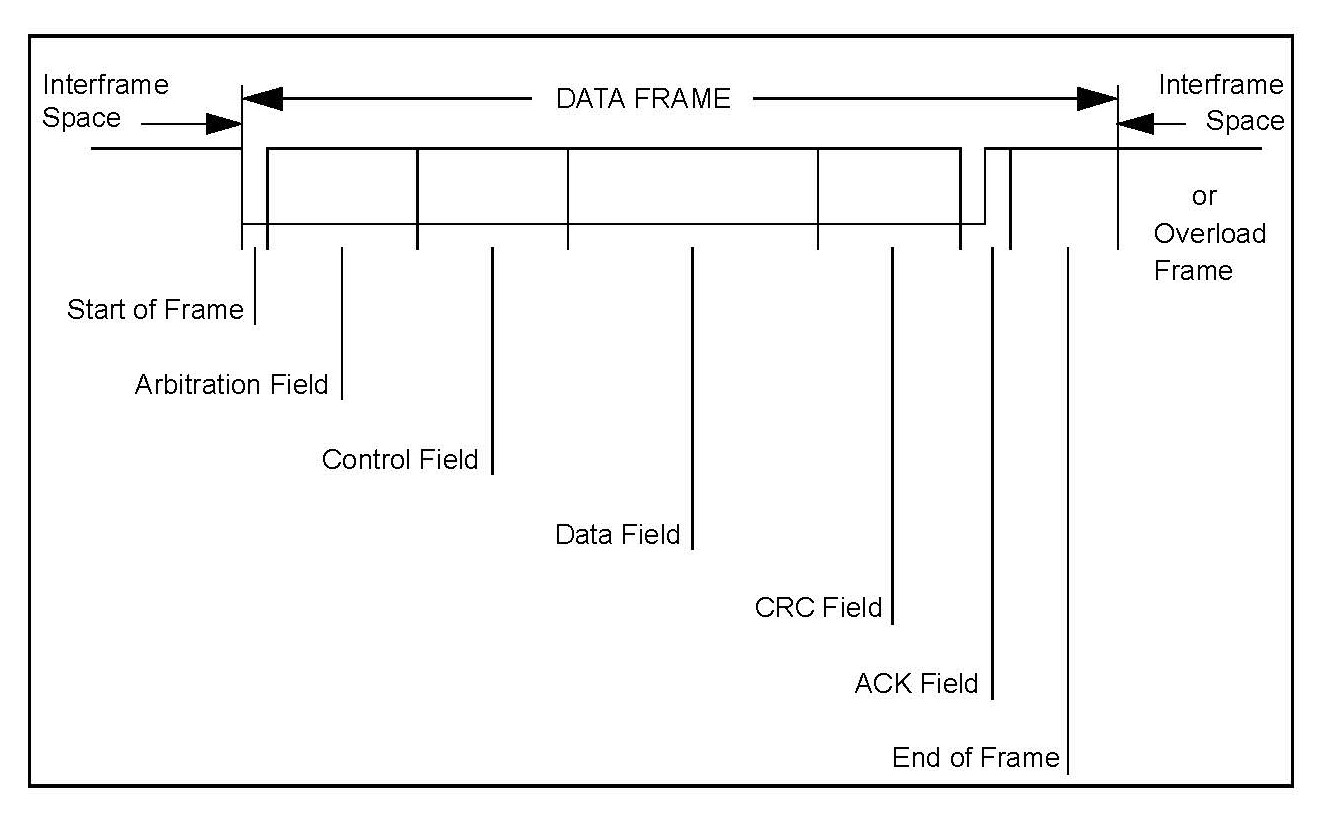
\includegraphics[width=\textwidth]{images/02-2023/CAN Specification_Page_11.jpg}
    \caption{(Bosch, 1991) A breakdown of the CAN message frame with all of the fields labeled.}
    \label{fig:can_specification}
\end{figure}
\pagebreak



\subsubsection{SocketCAN}
SocketCAN is a set of open source CAN drivers and a networking stack that provides a standardized Linux socket interface for accessing Controller Area Network (CAN) buses. It allows developers to communicate with CAN devices from user-space applications using standard socket APIs, which simplifies the development of CAN-based applications on Linux. SocketCAN has been included in the Linux kernel since version 2.6.25 and is widely used in industrial, automotive, and other embedded systems. The SocketCAN package is a Linux implementation of CAN protocols. It uses the Berkeley socket API and the Linux network stack; treating CAN device drivers as network interfaces. The framework provides a socket interface for user space applications and expounds upon the Linux network layer (CAN controller hardware device drivers are registered with the network layer as network devices, allowing CAN frames from the controller to be passed to the network layer. 
 \begin{figure}[!h]
    \centering
    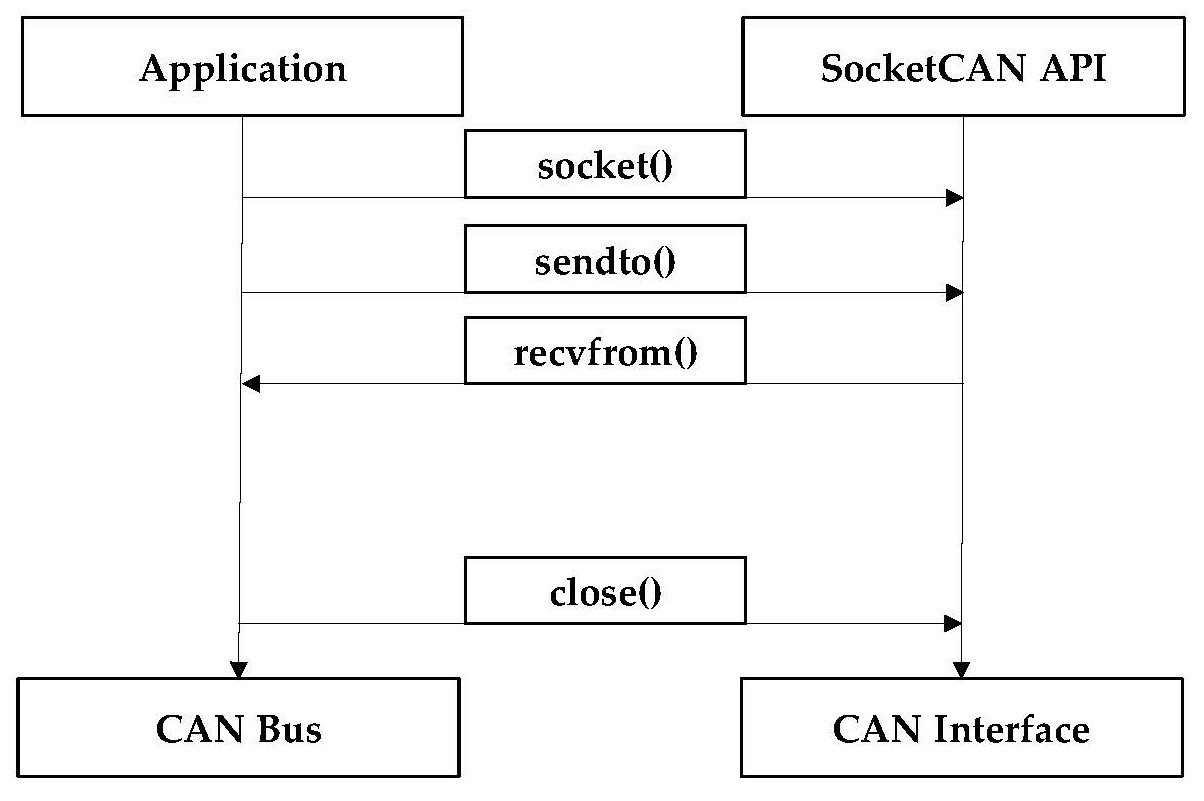
\includegraphics[width=\textwidth]{images/02-2023/SocketCAN.jpg}
    \caption{Application using SocketCAN API to communicate with CAN bus}
    \label{fig:can_specification}
\end{figure}
\pagebreak
In SocketCAN, functions can be used to configure and control the CAN interface and socket. The header libraries included provide definitions and declarations for the functions and data structures used in the API. The 'socket()' function is used to create a new SocketCAN socket that is bound to the CAN interface. The 'sendto()' function is used to send messages to the bus, and the 'recvfrom()' function is used to receive messages from the bus. After the application is finished using the socket, the 'close()' function releases the socket, freeing up associated resources. On the other side of the flowchart pictured above, the CAN interface communicates with the physical CAN bus (the interface hardware is responsible for transmitting and receiving messages on the bus). The SocketCAN driver in the Linux kernel provides a standardized interface accessing the CAN interface and controlling the flow of messages to and from the application.  Additional functions can be used to control the CAN interface and socket.
\subsubsection{CanKing}
Kvaser's CanKing is a Windows program for CAN bus monitoring and general-purpose diagnostics, particularly excelling as an interactive development and testing. Its features include:

\begin{multicols}{2}
\begin{itemize}
    \item Send/Receive CAN and Extended CAN messages
    \item Supports CAN FD, both ISO non-ISO
    \item Log to File (up to 4 channels)
    \item Filter Messages
    \item Generate Error Frames
    \item Timed Transmission 
    \item History Transmit List
    \item Traffic Generator 
    \item Virtual CAN Channels 
    \item Specify Custom Bus Parameters 
\end{itemize}
\end{multicols}

All of these features make it an invaluable tool for diagnostics and testing CANbus networks.

\subsubsection{USB2CAN}

\subsubsection{CANifier}
The CANifier is a CAN-controlled multipurpose LED and General Purpose Input/Output controller, used to "CANify" components of robotic control systems that typically do not utilize CAN bus. Its features include:

\begin{itemize}
    \item CAN bus controlled and field upgradable
    \item 3X LED channel drivers: Individual RGB control with 10bit resolution
    \item Outputs for common devices, including any PWM-controlled devices
\end{itemize}

\subsection{LoRa Communication} % Sydney and Humbi

Long Range, or LoRa, is a wireless communication technology that enables long-range, low-power communication between devices, particularly in Internet of Things (IoT) applications. 
It is a proprietary modulation technique developed by Semtech Corporation. 
LoRa operates in unlicensed ISM bands such as the 433 MHz and 915 MHz bands in the United States, and 868 MHz in Europe.
It uses spread-spectrum technology to communicate over long distances while consuming little power. 
The spread-spectrum modulation technique makes LoRa communication more resilient to interference. 
Its long-range capability allows devices to communicate over several kilometers, depending on the environment and line of sight. 
LoRa also employs a star network topology, where many end devices communicate with a single base station or gateway. 
The gateway acts as a bridge between the end devices and the network server, which can be connected to the internet. 
LoRaWAN is a network protocol built on top of LoRa technology, and it defines how LoRa devices communicate with the network server. 
LoRaWAN provides security, device management, and other features that are necessary for IoT applications, creating an inclusive ecosystem for connecting to and monitoring devices from anywhere in the world.

In robotics applications, commands can be sent from a command and control station far away from the vehicle.
The resiliency of LoRa allows for a strong connection over long distances and decreases the likelihood of communications faults due to interference.
However, the low data rate hinders operator's options for sending and receiving telemetry.
For instance, video streams are not possible with a LoRa connection as they require too much bandwidth.

\subsection{Sensing and Models}
    USVs have to be able to understand themselves and their surroundings in order to operate effectively.
    There are two types of models that semi- or fully-autonomous systems must be able to construct online (in real-time): the world model, and the local model.
    
    The world model represents all of the external factors that affect the USV's operation.
    This includes other ship traffic, weather, water conditions, obstructions, landmarks, GPS coordinates, operator commands, etc.
    Typically, the USV will build a world model by fusing different data streams together to formulate a best guess of its surroundings.
    If, for example, we have an AIS radio that tells the USV other ships' positions and trajectories, we can fuse that information with RADAR tracks and superimpose them together.
    Not all ships may be transmitting AIS, so we need RADAR to actively spot and track them; conversely, not all ships may appear properly on RADAR, but their AIS signals will allow the USV to estimate their position.
    By fusing these two data streams together, the USV can have a highly confident estimation of the traffic around it and maneuver accordingly.

    Similarly, the USV has to understand its internal data to understand its own capabilities and limitations.
    Sensors like strain gauges, voltage monitors, ammeters, accelerometers, fuel gauges, etc. all feed data to the USV's central computer to inform it of its own health.
    In our particular case, we want to limit the power consumption of the vehicle to maximize efficiency.
    We can integrate a power distribution board that reports the voltage levels and power consumption of various channels to the USV's computer.
    The computer can then monitor the power draw of the entire system and calculate an estimated battery charge remaining based on the time interval and battery discharge model.
    If the system is drawing too much power, the computer can order subsystems to ramp down usage or vice versa.
    An accurate local model will be an additional layer of security that ensures SEACAT will be able to complete the course with remaining power and without damaging components.    

\section{Trailer Updates} % Jackson and Alex
As the home base of the command and control center, the trailer must provide electric power to the controls and a practical working space for at least two users. 
A gasoline-powered generator will produce the electricity required by the trailer. 
The output wattage is governed by the electricity demand of the trailer and control system's components. 
The largest power draw of the trailer will be the air conditioning unit which will be required for pilots to use the trailer in high outdoor temperatures. 
The trailer's projected AC unit will require about 1,500 Watts to run. 
Other electrical equipment, including the computer communicating with SEACAT, can be expected to draw a couple hundred more Watts. 
The generator, therefore, will have a minimum power output of 3,300W which will provide sufficient power with about a factor of safety of two.

\subsection{Proposed Design}

\begin{figure}[h!]
    \centering
    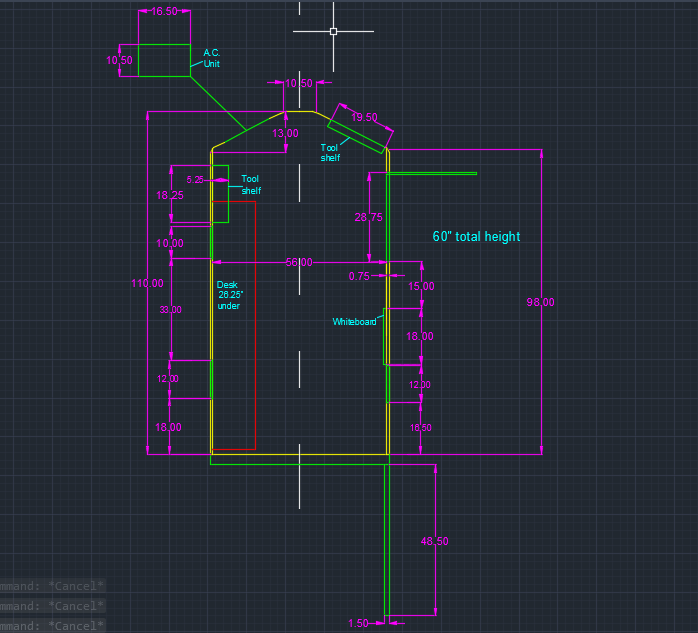
\includegraphics[width=10cm]{images/02-2023/trailer/Trailer Schematic.png}
    \caption{Trailer Schematic}
    \label{fig:my_label}
\end{figure}

\subsection{Current Status}
Prior to being adopted by the PANTHER team, the trailer had not been moved in several years. Neglect has left the trailer in need of replacing the axles and the wheels due to corrosion. Upon further inspection, there are potential structural issues in the floor supports after years of rust have left them brittle. The old air conditioning unit is still installed in the trailer, and it will be removed when a new unit can replace it. In February, the team completely cleaned the trailer out to prepare to take it to the shop for maintenance and repairs. After structural repairs are made, the team must check on the validity of any electric wiring currently installed in the trailer. Once the repairs are made, the team will be able to begin the renovation and refitting of the trailer into a proper command center.  
\subsection{Fabrication Timeline}

\begin{itemize}
    \item The trailer progress is currently at a halt due to paperwork backup. Without an updated registration, the trailer is immovable and cannot be taken to a shop for repair. There is no projected date for the paperwork to be completed at the moment. 
\end{itemize}

\section{Naval Architecture Updates} % Cannon, Jackson and Humbi

\subsection{Models}


This section presents the naval architecture aspect of SEACAT, the fully electric catamaran. 
SEACAT is a multi-hull catamaran. 
The hulls are fiber glass of length 66.2" and width 8". 


\begin{table}[h!]
\centering
    \begin{tabular}[c]{| c | c |}
    \hline
    \multicolumn{2}{| c |}{Hull Dimensions}\\
    \hline
    Length & 66.2"\\
    \hline
    Beam & 8" \\
    \hline
    Weight & 13 lbs \\
    \hline
    
    \end{tabular}
    \caption{Table : Demi-Hull Parameters.}
    \label{Table:1}
\end{table}

\begin{figure}[h!]
    \centering
    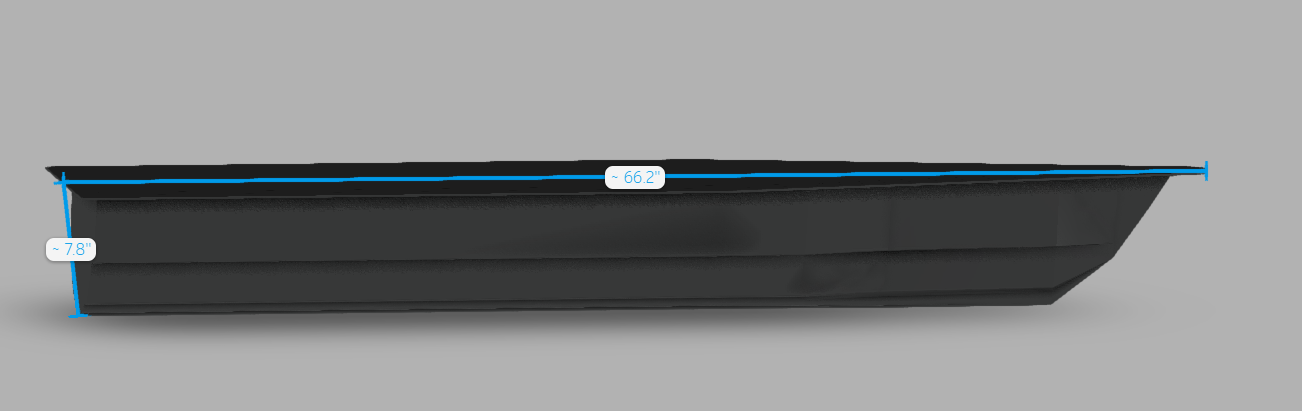
\includegraphics[width=10cm]{images/02-2023/hull/Demihull2}
    \caption{Demi-hull Design}
    \label{fig:my_label}
\end{figure}

Initial CAD design for the hulls were made using Fusion 360 software, from were it was imported into Rhino7 for further analysis. Rhino7 provides the users with tools for Naval Architecture such as Orca3D. Which provides the ability to adjust the hull design, while given the ability to do Hydrostatics \& Stability and Speed \& Power analysis. Speed \& Power analysis guided the team in the correct route to select the initial motors for testing, by providing the power needed to go at a desired speed. Last but not least Rhino7 provides a combination between Orca3D and Simerics CFD (Computational Fluid Dynamics).

Initial CFD simulations were performed using ORCA3D and Simmerics to obtain the Effective Horse Power (EHP) and Resistance curves of the catamaran. The simulations were carried out under different design conditions first at 80 pounds, then at 60 pounds and finally at 55 pounds. During the 80 pounds simulation it was found that the sinkage (5.5 in) of the hulls was over the safe limit (4.5 in), to mitigate this it was decided that a re-adjustment of weight was needed. The new max weight is 60 pounds with the reach goal to achieve 55 pounds. CFD simulations were carried at various speeds from 10 to 16 knots with a 2 knot step size. The simulations account for the entire catamaran and the surrounding water. The resistance and EHP curve are presented in Figure 6 and 7, respectively. While hydrostatics parameters can be found in table 2.
An important aspect to note is that we are not presenting all the results obtained, only presenting the best results. This is due to instability in the system after 12 knots of speed. After this speed the EHP curve would keep oscillating and does not reach a steady state. A tow test is being plan to corroborate some of the results oftained from the CFD. 

\begin{table}[h!]
\centering
    \begin{tabular}[c]{| c | c |}
    \hline
    \multicolumn{2}{| c |}{Volume Properties}\\
    \hline
    Displacement & 60 lbf\\
    \hline
    Total displaced volume & 0.95 ft3\\
    \hline
    Sinkage & 4.45 in \\
    \hline
    Block Coefficient & 0.176 in \\
    \hline
    LCB & 26.938 in \\
    \hline
    Wet Area & 9.22 ft2 \\
    \hline
    Draft & 3.12 in\\
    \hline

    \end{tabular}
    \caption{Table : Hydrostatics Parameters.}
    \label{Table:2}
\end{table}


\begin{figure}[h!]
    \centering
    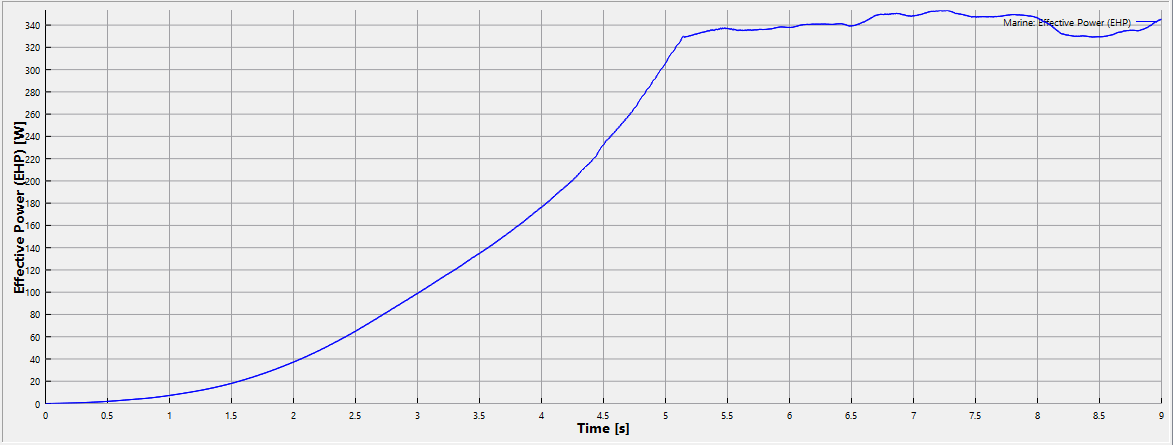
\includegraphics[width=10cm]{images/02-2023/cfd/60 lbs/ehp 10 knots}
    \caption{EHP curve}
    \label{fig:my_label}
\end{figure}

\begin{figure}[h!]
    \centering
    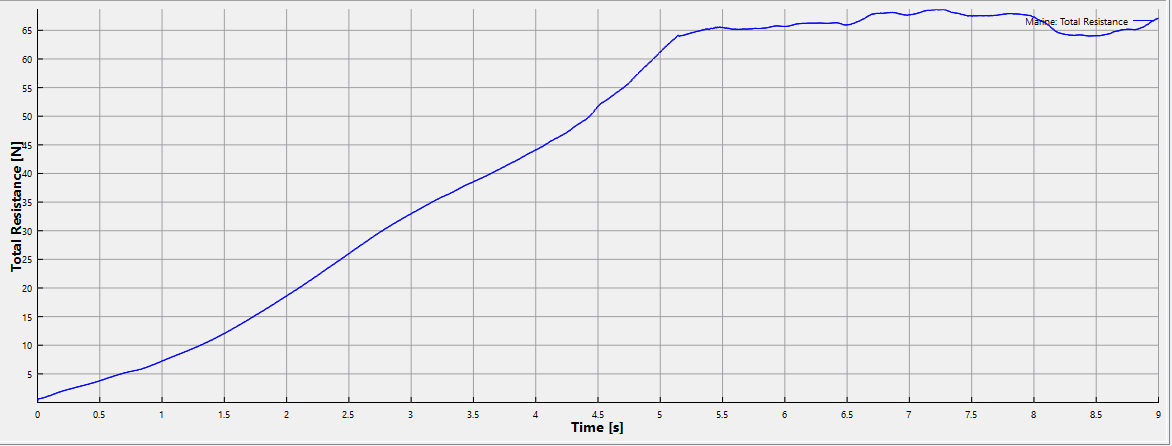
\includegraphics[width=10cm]{images/02-2023/cfd/60 lbs/resistance}
    \caption{Resistance curve}
    \label{fig:my_label}
\end{figure}

The EHP curve show the power required to achieve a certain speed with minimum power consumption, this power is the required to overcome the resistance of the catamaran. From figure 6 we observe that the lowest required power is at a speed of 10 knots, this is the optimal speed and weight obtained from the simulations results.From the resistance and power analysis we confirmed that has weight and/or speed increases the power required will proportionally increase as well. 

During the process of iterating between different weights and speed we found that at 55 pounds running at 10 knots we obtain the optimal energy consumption. Figures 8, 9, and 10 show the EHP curve, resistance curve and a visual representation of the forces acting in the hull, respectively. Has a reach goal the team is looking into efficient ways of no exceeding a maximum weight of 55 pounds for the whole boat. 


\begin{figure}[h!]
    \centering
    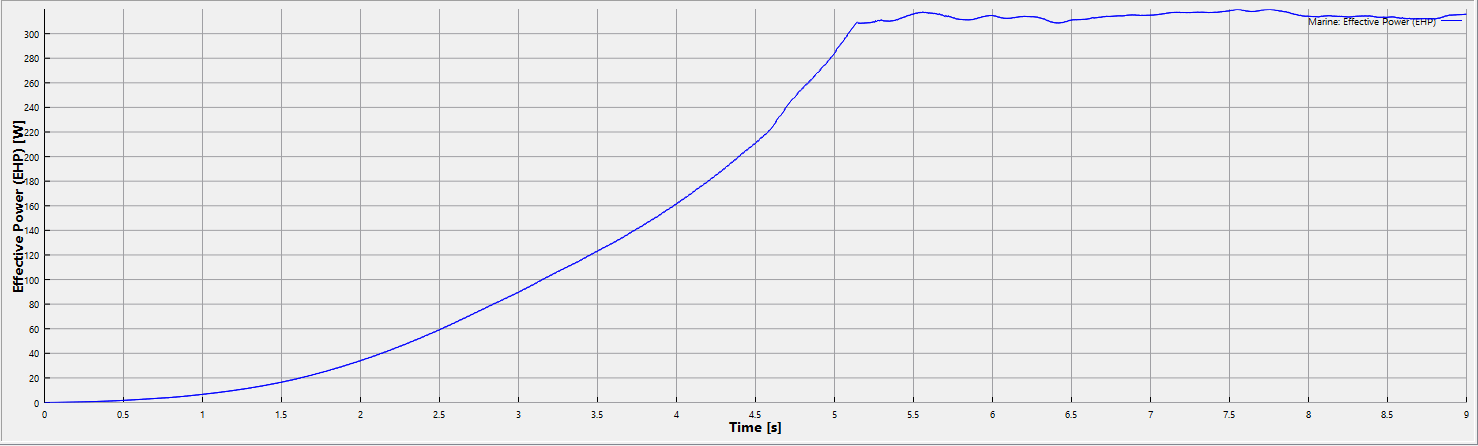
\includegraphics[width=10cm]{images/02-2023/cfd/55 lbs/EHP_10 knts}
    \caption{EHP curve}
    \label{fig:my_label}
\end{figure}

\begin{figure}[h!]
    \centering
    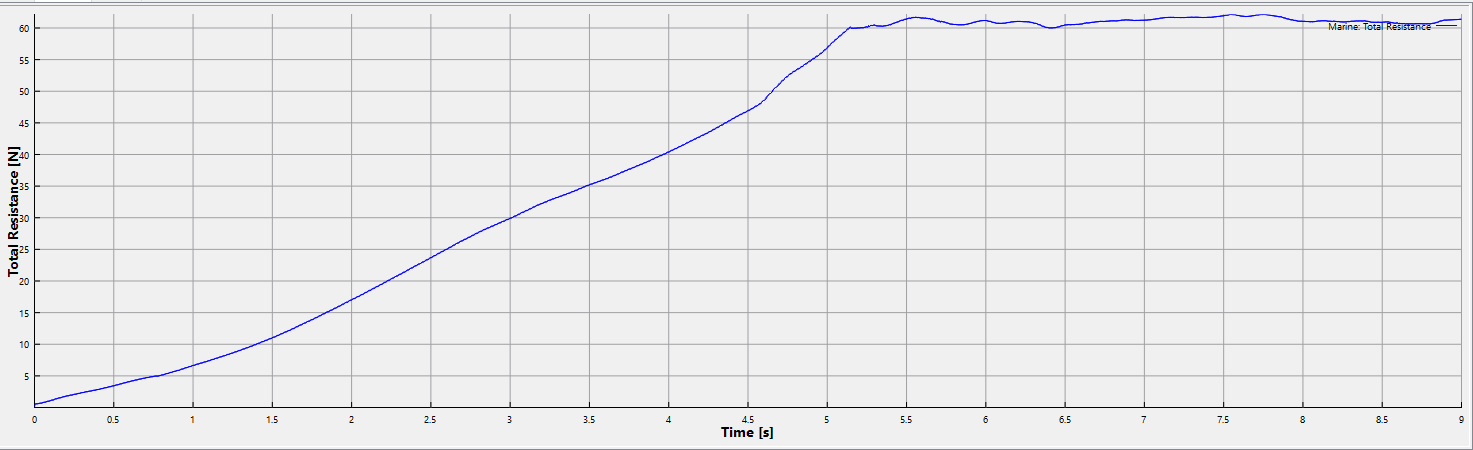
\includegraphics[width=10cm]{images/02-2023/cfd/55 lbs/Resistance_10_knts}
    \caption{Resistance curve}
    \label{fig:my_label}
\end{figure}

\begin{figure}[h!]
    \centering
    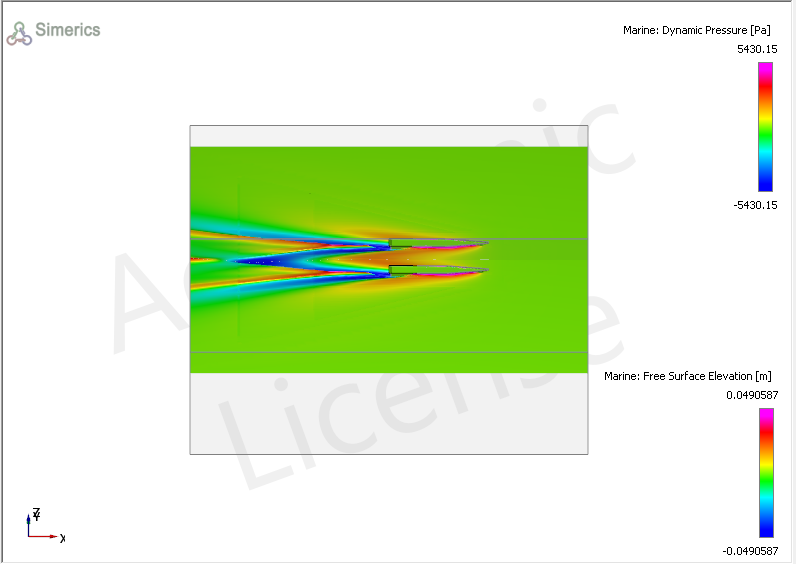
\includegraphics[width=10cm]{images/02-2023/CFD/55 lbs/Graphs_10knts}
    \caption{Visual Representation force acting on hulls}
    \label{fig:my_label}
\end{figure}

Further analysis are to be done such as Efficiency \& Range Analysis, Power Consumption Analysis and Seakeeping Analysis. As for the boat model a body plan of the hulls is to be design. 



\subsection{Electrical/Mechanical Systems Progress} 
From the EHP curve we obtained the required power needed for the catamaran to move at [knots] with a 50\% efficiency from the propulsion system.The F4125 300KV 410W brushless motor for Direct Drive Propeller/Efoil were bought for initial testing. The F4125 300KV provide a maximum of [410 watts]. Has a starting point..... 

\subsection{Motor/Propeller Selection/Design Progress}
SeaCAT’s Motor choice and the design methods were based on size constraints within the boat hulls. The Motors were chosen dependent on the size and speed required to run 5 miles at a fast and controlled rate. The motors need to fit in a 2x3 space in between both hulls. At this early point in the design phase we are approximating the boat to weigh about 60-80 lbs when its complete. We will use the weight and distance to calculate how fast we need the boat to move to hit the time we're requiring to win, aiming to beat last years winner at 17 minutes. Once we have that time calculated out, we will determine the battery size and wattage required for our appropriate torque calculation and power necessary. We aim for quick acceleration of the SEACAT and aim to stay buoyant without capsizing during the fixed turns in the race.
Pantherboat does not suspect any unknown turns to factor into our calculations.

\pagebreak

\subsection{Specs Electric}
Important Specs currently for the boat model are:
\begin{itemize}
    \item Maximum power:410W
    \item Motor diameter: 46mm
    \item Motor length: 50mm
    \item Shaft diameter: 4.85mm
    \item Torque: 0.9N.m
    \item Weight:310g
    \item Motor Dynamics - During our preliminary design planning, some experimental motor testing was conducted with a small 6 V Battery and several small 12 V DC brushless motors were used to model what we would ideally need when CADing adaptors,shaft fixtures, and slip rings when connecting the motor,shaft, and propellers to best fit our needs. This was the first step accomplished before our actual boat motor was purchased
\end{itemize}



\begin{itemize}
    \item Contingencies and Considerations
-that are now being considered during motor selection, are determining the lightest amount the hull model can be.     
There were some other motor considerations in the final decision processes but the limiting factors was price and availability.
\end{itemize} 

\subsection{Vehicle Properties and Dynamics Testing}

\begin{itemize}
    \item Tow Testing - To corroborate some of the CFD results, a tow testing has been schedule. By towing the boat we can compare experimental results with our CFD results. [Explain the set-up we are going to use]
    
    \item Propulsion Testing - 
    
Having selected our whole initial propulsion system at this point.

    \end{itemize}


\section{Works Cited} (Mary)
\pagebreak

\end{document}